\chapter{Materiais e Softwares}
% ---
Nas seções a seguir são apresentados os \textit{hardwares} e \textit{softwares} utilizados na construção do sistema proposto.
% ---
\section{Microcontroladores e Microprocessadores}
% ---

Buscando aumentar a eficiência no processamento de dados, na década de 70
começaram a ser utilizados microprocessadores em computadores \cite{martins2005sistemas}. Os microprocessadores são componentes dedicados ao processamento de informações com
capacidade de cálculos matemáticos e endereçamento de memória externa \cite{chase2007sistemas}.

Por sua vez, os microcontroladores são pequenos sistemas computacionais poderosos que englobam em um único chip: interfaces de entrada/saída digitais e analógicas, memória RAM, memória FLASH, interfaces de comunicação serial, conversores analógicos/digitais, temporizadores/contadores e um microprocessador \cite{chase2007sistemas}.

Na Figura \ref{fig:microprocessador-microcontrolador}, pode-se observar algumas das diferenças entre Microprocessadores e Microcontroladores. O microcontrolador embarca todos os componentes necessários ao seu funcionamento, enquanto o microprocessador precisa de comunicar externamente com os periféricos similares.

\begin{figure}[htbp]
	\centering
	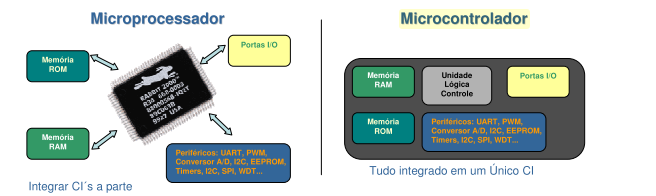
\includegraphics[scale=0.7]{figuras/processa-controla.png}
	\caption{Arquitetura básica de microprocessadores e microcontroladores.}
	\legend{Fonte: \citeauthor{chase2007sistemas} (\citeyear{chase2007sistemas})}
	\label{fig:microprocessador-microcontrolador}
\end{figure}

\newpage

%O microcontrolador a ser utilizado no projeto é o ESP8266 (Figura \ref{fig:esp}), que é um circuito integrado, com interfaces de I/O digitais e analógicas. Possui interface Wi-Fi, com um microprocessador de 32 bits, capaz de executar tarefas a 160 MHz.
%
%Os circuitos baseados no microcontrolador ESP8266 representam um grande avanço na relação de preço-recursos e pode ser um componente muito interessante para soluções IoT \cite {de2017internet}.
%
%\begin{figure}[htbp]
%		\centering
%		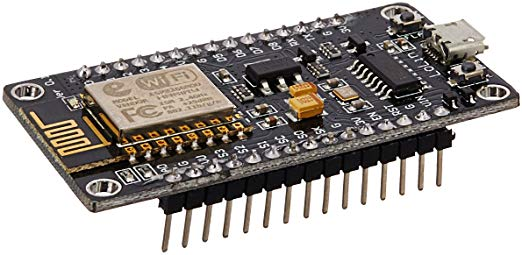
\includegraphics[scale=0.5]{figuras/esp8266_.jpg}
%		\caption{ESP8266.}
%		\legend{Fonte: \citeauthor{Kodali2017} (\citeyear{Kodali2017})}
%		\label{fig:esp}
%\end{figure}


\subsection{Raspberry Pi}

O Raspberry Pi (Figura \ref{fig:rpi}) é um minicomputador criado pela Raspberry Pi Foundation. Seu objetivo é estimular o ensino da ciência da computação nas escolas e universidades. Apesar do Raspberry Pi possuir o hardware em uma única placa eletrônica de tamanho reduzido, seu potencial de processamento é significativo \cite{crotti2013raspberrypi}. O Raspberry Pi pode ser usado em diversos projetos tecnológicos, como experimentos remotos nos quais sua função é ser um micro servidor web \cite{crotti2013raspberrypi}.

\begin{figure}[htbp]
		\centering
		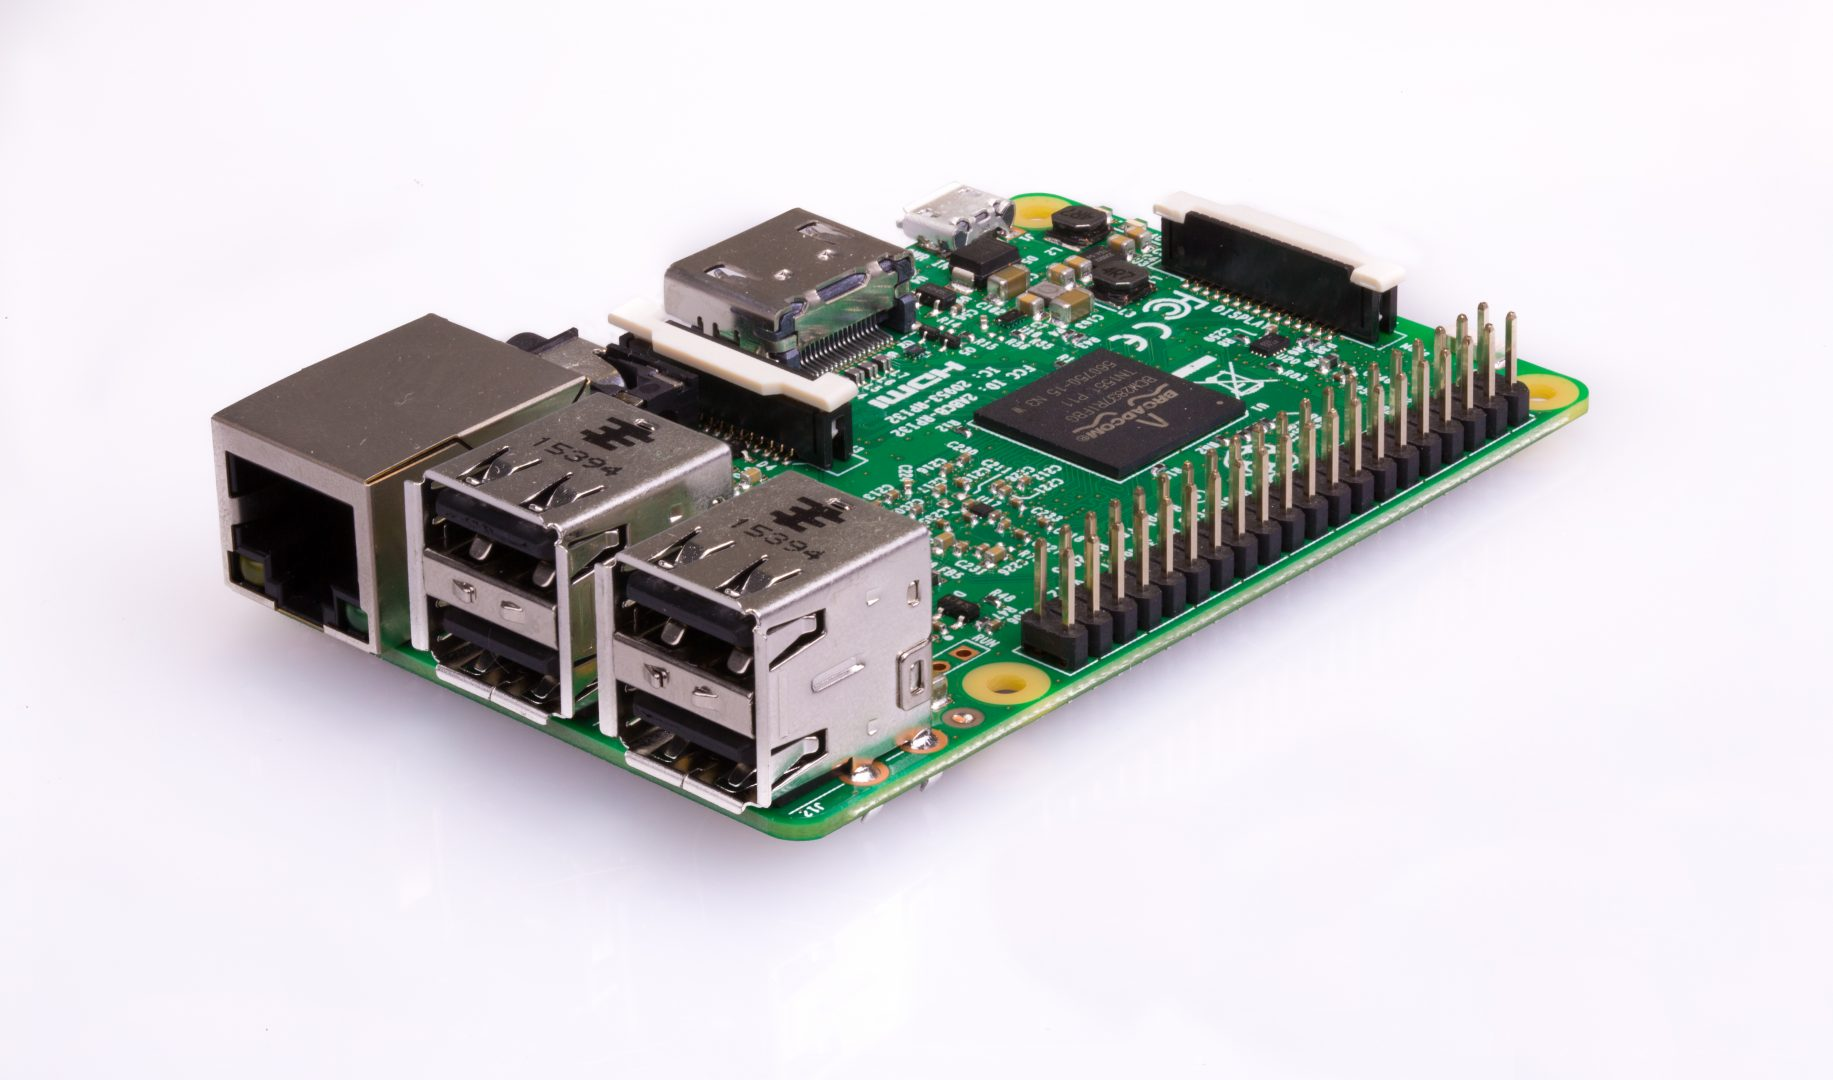
\includegraphics[scale=0.2]{figuras/raspberrypi.jpg}
		\caption{Raspberry Pi.}
		\label{fig:rpi}
\end{figure}

\section{Sensores e atuadores}

Nesta seção serão apresentados os sensores e atuadores a terem seus sinais utilizados no projeto. 

\subsection{Sensor de fluxo YF-S201} \label{sec:sensor}

O sensor YF-S201 (Figura \ref{fig:sensor}) é um sensor do tipo turbina que mede a quantidade de líquido que passa pela tubulação, girando aletas que
geram pulsos de onda quadrada através de um sensor de efeito Hall \cite{roque2018sistema}. O
sensor usa esse efeito para enviar um sinal PWM (\textit{Pulse Width Modulation}) e, através da contagem deste sinal é possível mensurar a quantidade de água que passa pela turbina no interior do sensor. \cite{ms2017automaccao}

\begin{figure}[htbp]
		\centering
		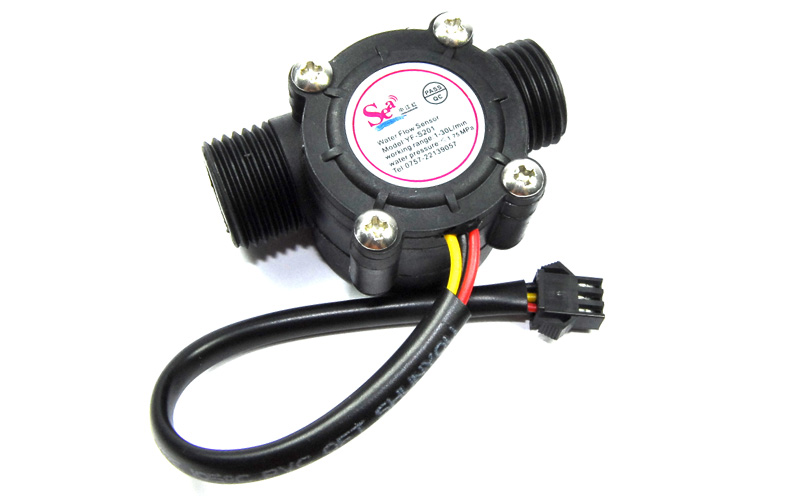
\includegraphics[scale=0.3]{figuras/yf-s201.jpg}
		\caption{Sensor de fluxo de água YF-S201.}
		\label{fig:sensor}
\end{figure}

\newpage

\subsection{Teclado matricial de membrana} \label{sec:teclado}

Teclados permitem que usuários insiram informações em diversos tipos de sistemas, como computadores, calculadoras, controles remotos entre outros \cite{teclado-matricial-1}. O Teclado Matricial de Membrana 4X4 (Figura \ref{fig:teclado}) foi desenvolvido com a finalidade de facilitar a entrada de dados em projetos com plataformas microcontrolada \cite{teclado-matricial}. Este teclado possui 16 teclas, sendo 10 teclas são numéricas, 4 literais e 2 caracteres especiais.

\begin{figure}[htbp]
	\centering
	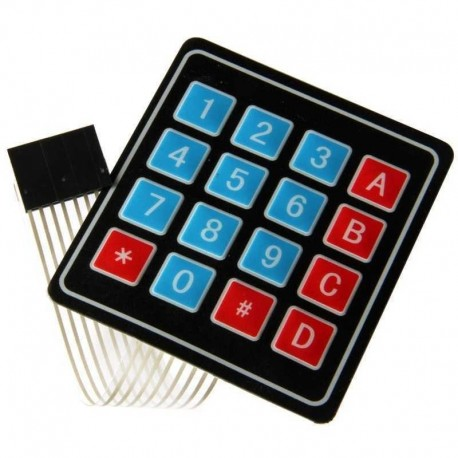
\includegraphics[scale=0.2]{figuras/teclado-matricial.jpg}
	\caption{Teclado Matricial de Membrana.}
	\legend{Fonte: \citeauthor{teclado-matricial-1} (\citeyear{teclado-matricial-1})}
	\label{fig:teclado}
\end{figure}

As teclas estão dispostas em 4 linhas por 4 colunas e o teclado possui um conector de 8 pinos para ligação. Quando um botão do teclado é pressionado, ele conecta a linha com a coluna na qual está ligado, gerando um sinal nos pinos referente àquela linha/coluna. Este sinal permite a identificação da tecla apertada pelo sistema. O circuito do teclado está exemplificado na Figura \ref{fig:teclado-conexoes}.

\begin{figure}[htbp]
	\centering
	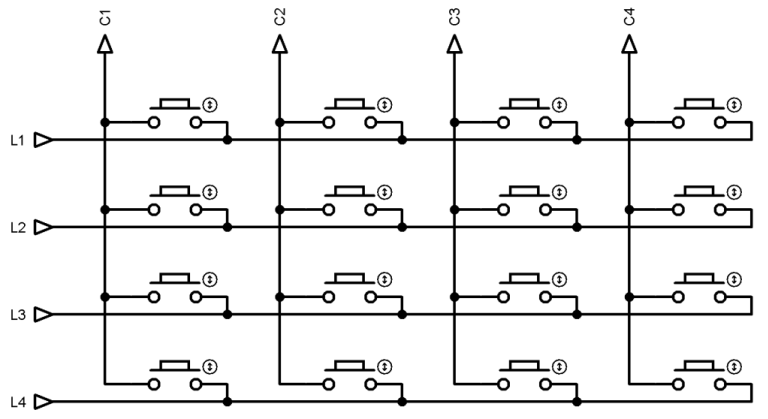
\includegraphics[scale=0.4]{figuras/matrix-1024x558.png}
	\caption{Circuito do teclado.}
	\legend{Fonte: \citeauthor{teclado-matricial} (\citeyear{teclado-matricial})}
	\label{fig:teclado-conexoes}
\end{figure}

A Tabela \ref{table:pinosteclado} possui as informações da distribuição dos pinos em tabelas e colunas, exemplificada na Figura \ref{fig:teclado-pins}.

\begin{table}[h!]
	\begin{center}
		\begin{tabular}{ |c|c| }
			\hline
			\rowcolor{lightgray} Pino & Localização \\
			 \hline 
				1 & Linha 1 \\
			 \hline 
				2 & Linha 2 \\
			 \hline 
				3 & Linha 3 \\
			 \hline 
				4 & Linha 4 \\
			 \hline 
				5 & Coluna 1 \\
			 \hline 
				6 & Coluna 2 \\
			 \hline 
				7 & Coluna 3 \\
			 \hline 
				8 & Coluna 4 \\
			\hline
		\end{tabular}
	\caption{Tabela de disposição dos pinos do teclado numérico.}
	\label{table:pinosteclado}
	\end{center}
\end{table}

\begin{figure}[htbp]
	\centering
	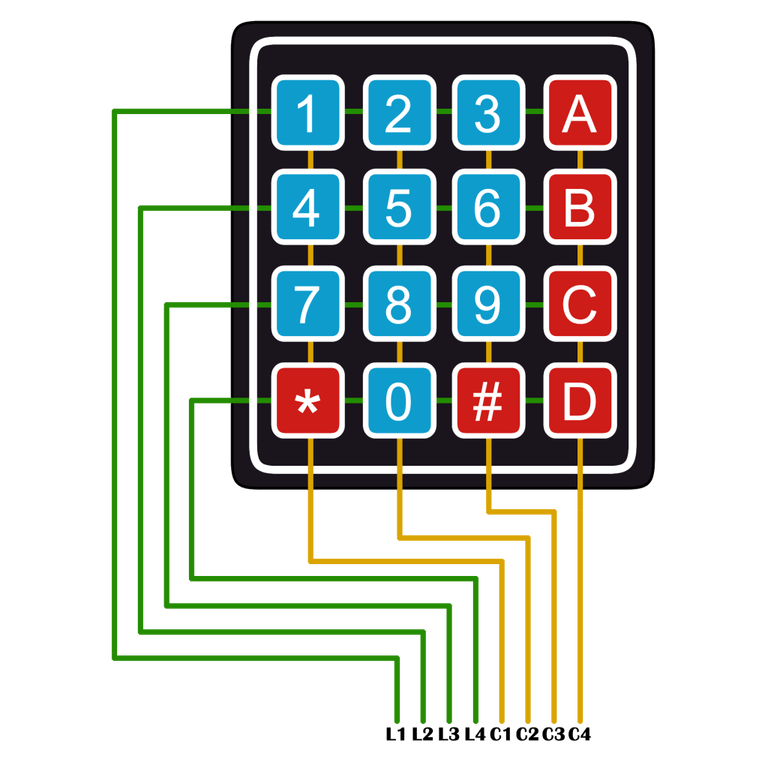
\includegraphics[scale=0.3]{figuras/keypad-1024x1024-pins.png}
	\caption{Pinagem do teclado.}
	\legend{Fonte: \citeauthor{teclado-matricial} (\citeyear{teclado-matricial})}
	\label{fig:teclado-pins}
\end{figure}

\newpage

\subsection{Válvula solenoide} \label{sec:valvula}

Solenóides são dispositivos eletromecânicos baseados no deslocamento causado pela ação de um campo magnético gerado por uma bobina e são muito utilizados na construção de outros dispositivos, como é o caso das válvulas para controle de fluidos. Em particular, as válvulas para baixas vazões (da ordem de mililitros por minuto) e baixas pressões têm sido amplamente aplicadas em equipamentos e montagens para uso em laboratórios clínicos e químicos  \cite{da2002modulo}. Elas são de pequenas dimensões e requerem baixa tensão e corrente de acionamento.

A válvula solenoide pode ser vista na Figura \ref{fig:valvula-solenoide}.

\begin{figure}[htbp]
	\centering
	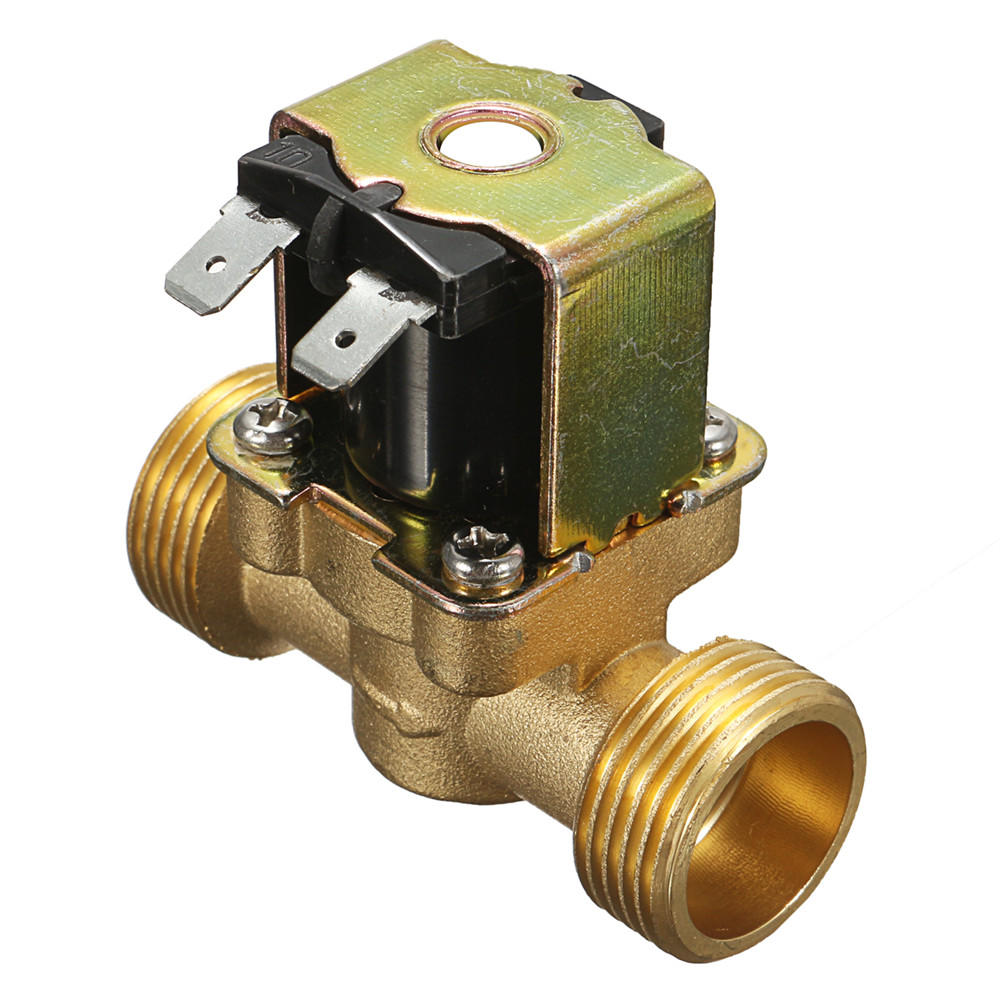
\includegraphics[width=0.3\linewidth]{figuras/valvula-solenoide.jpg}
	\caption{Válvula Solenoide.}
	\label{fig:valvula-solenoide}
\end{figure}

Segundo \citeauthor{da2002modulo} (\citeyear{da2002modulo}), a estratégia para fechamento e abertura dos canais fluídicos depende do fabricante, mas o princípio de acionamento elétrico é comumente o mesmo. Uma tensão é aplicada sobre um solenoide, criando um campo magnético que desloca um núcleo ferromagnético móvel, causando a alteração do estado da válvula. O núcleo
ferromagnético comprime uma mola que é a responsável por retornar o núcleo a sua posição original quando a corrente elétrica é interrompida.

\section{Softwares}

Os softwares que foram utilizados para a implementação do sistema estão presentes nesta seção.

\subsection{HomeAssistant}

O HomeAssistant é um plataforma de automação escrita em Python. Inclui componentes contribuídos por usuários que permite a interface com Web Services e dispositivos como sensores, microcontroladores e assistentes virtuais \cite{Lundrigan2017}. Em seu núcleo, o HomeAssistant é um protocolo de troca de mensagens que facilita a comunicação entre dispositivos e componentes funcionais na rede. Provendo simples abstrações de componentes de automação residencial como sensores, câmeras, \textit{players} de música, etc.

A Figura \ref{fig:homeassistant-dash} apresenta um exemplo de tela inicial do HomeAssistant. Com vários sensores configurados na parte superior, na parte esquerda, encontra-se o menu do HomeAssistant, e na parte central inferior pode-se observar informações sobre o clima e \textit{switches} para acionamento de interruptores e iluminação.

\begin{figure}[htbp]
	\centering
	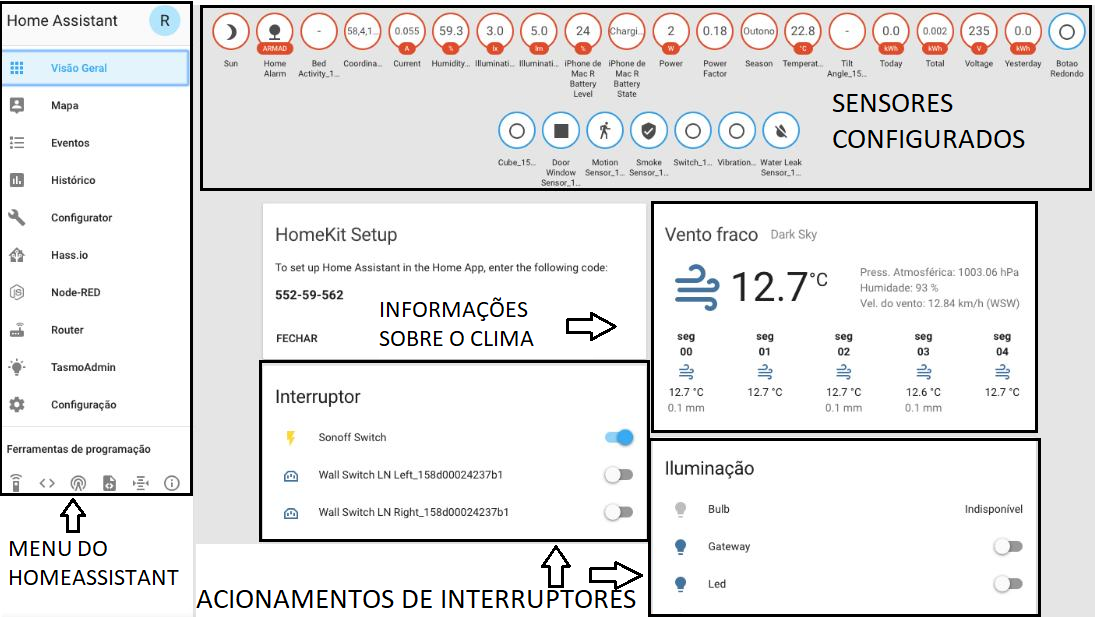
\includegraphics[width=1\linewidth]{figuras/homeassistant-dash.png}
	\caption{Dashboard genérico do HomeAssistant}
	\legend{Fonte: Adaptado de \citeauthor{AlmeidaCosta} (\citeyear{AlmeidaCosta})}
	\label{fig:homeassistant-dash}
\end{figure}

O HomeAssistant tem suporte para diversos tipos de protocolos \textit{wireless}, como BLE, ZigBee, Z-Wave e Wi-Fi. Conta também com um RESTful API e suporta HTTP, MQTT, TCP \textit{sockets} e componentes customizados. Estes componentes customizados permitem aos usuários adicionar funções próprias no HomeAssistant sem a necessidade de mudar o seu código fonte. Isto torna a integração de novos dispositivos e sensores muito mais fácil com o HomeAssistant \cite{Gomes2018}.


%O HomeAssistant conta com uma grande comunidade de desenvolvedores com mais de 1.450 contribuidores e 23.700 estrelas no GitHub\footnote{\url{https://github.com/home-assistant/home-assistant}}, o que significa uma abundância em sua documentação sobre os seus componentes, fóruns e chats para conseguir ajuda de outros usuários, e diversos posts em blogs e vídeos sobre como começar a utilizar o programa.

Tendo em vista a gama de protocolos sem fio disponíveis no HomeAssistant, escolhemos o padrão Wi-Fi pois segundo \citeauthor{Lundrigan2017} (\citeyear{Lundrigan2017}):

\begin{itemize}
	\item O custo dos equipamentos com padrão Wi-Fi é reduzido.
	\item Wi-Fi é o mais difuso dos protocolos wireless.
	\item Sensores Wi-Fi tem integração facilitada com demais equipamentos residenciais.
\end{itemize}

O HomeAssistant pode ser instalado em qualquer sistema operacional devido ao fato de ser muito pequeno e leve. O que o faz ser compatível para o uso no Rasberry Pi como um hub de automação pequeno e barato. É importante lembrar que o HomeAssistant age apenas como uma central de controle que pode informar outros serviços, como o Philips Hue ou o Nest, que são produtos para automação residencial, para realizar alguma função \cite{AlmeidaCosta}. O Home Assistant é gratuito e de fácil configuração.

\subsection{Banco de dados de séries temporais}

Um Banco de Dados de Séries Temporais, do inglês \textit{Temporal Series Database} (TSDB), é um tipo de banco otimizado para dados coletados no tempo. É implementado especificamente para lidar com métricas, eventos ou medidas que variam no tempo. Um TSDB permite o usuário criar, enumerar, alterar, destruir e organizar várias séries temporais de métodos mais eficientes. Atualmente, a maioria das empresas estão gerando um grande volume de dados sobre métricas e eventos que são mapeados no tempo, aumentando a relevância de tal arquitetura \cite{Noor2017}.

Ainda segundo \citeauthor{Noor2017} (\citeyear{Noor2017}), aplicações comuns para os TSDBs são IoT, DevOps e Analise de Dados. Alguns casos de uso incluem monitoramento de sistemas de \textit{software} como máquinas virtuais, monitoramento de sistemas físicos como dispositivos, ambiente, sistemas de automação residencial, dentre outros.

\subsubsection{InfluxDB}

O InfluxDB é o Banco de Dados de Séries Temporais usado neste projeto, sendo o mais apto a guardar os dados de fluxo no tempo. \cite{Lundrigan2017}

É um projeto \textit{open-source} com o opcional de armazenamento pago em nuvem desenvolvido pela empresa InfluxData. É escrito na linguagem de programação Go e baseado em uma linguagem de consulta parecida com o SQL \cite{Noor2017}.

\subsubsection{Grafana}

Grafana é um projeto \textit{open-source} para análise de dados de séries temporais  \cite{Noor2017} que realiza consultas destas séries temporais a partir do InfluxDB exibindo os dados de maneira gráfica \cite{chang2017kubernetes}.

\subsection{Banco de dados relacional}

Um Banco de Dados Relacional é capaz de salvar e referenciar dados para uma consulta posterior. Possui uma coleção de tabelas, todas com identificadores únicos, que compõem a base de
dados. Conceitos como integridade referencial de dados – que garante sincronia de dados entre tabelas – e chaves primárias estão presentes, garantindo que um conjunto de informações possa ser representado de maneira consistente, independente da forma de acesso  \cite{bancosrelacionais}.

\subsubsection{PostgreSQL}

O PostgreSQL é uma implementação de um banco de dados relacional, de código aberto e de custo gratuito \cite{stones2006beginning}. O 
PostgreSQL pode ser usado com diversas linguagens de programação, como por exemplo: Python, Javascript, Java e C++.

O PostgreSQL ganhou diversos prêmios, incluindo o \textit{Linux Journal Editor's Choice Award for Best Database} três vezes e o \textit{2004 Linux New Media Award for Best Database System}.

\subsection{Node.JS}

O Node.JS, também chamado de Node, é um ambiente de servidor que utiliza a linguagem de programação JavaScript. É baseado no \textit{runtime} do Google, chamado de motor V8. O V8 e o Node são implementados em C e C++, focados no desempenho e baixo consumo de memória. Embora o V8 suporte principalmente o uso de JavaScript no navegador, o Node foca no suporte de processos de servidores \cite{Tilkov2010}.

O Node.JS utiliza um paradigma baseado em eventos e não-bloqueador de I/O, o que o torna leve e eficiente. É perfeito para aplicações de tempo real que lidam com dados intensos em dispositivos de baixo poder de processamento \cite{Sapes2016}.

O Node é um dos ambientes e \textit{frameworks} mais famosos que suportam o desenvolvimento de servidores utilizando o JavaScript. A comunidade criou um grande ecossistema de bibliotecas e vasta documentação de suporte ao Node \cite{Tilkov2010}.

\subsection{Arquitetura de microsserviços}

Seguindo a definição de \citeauthor{ms1} (\citeyear{ms1}), a arquitetura de microsserviços trata do desenvolvimento de uma aplicação que baseia na existência de diversos pequenos serviços independentes. Cada um dos serviços deve rodar em seu próprio processo independente. Estes serviços podem comunicar entre si utilizando mecanismos leves de comunicação (geralmente em torno no HTTP). Os serviços devem ser absolutamente independentes.

Um exemplo da arquitetura de microsserviços está na Figura \ref{fig:arquitetura-microsservicos}.

\begin{figure}[htbp]
	\centering
	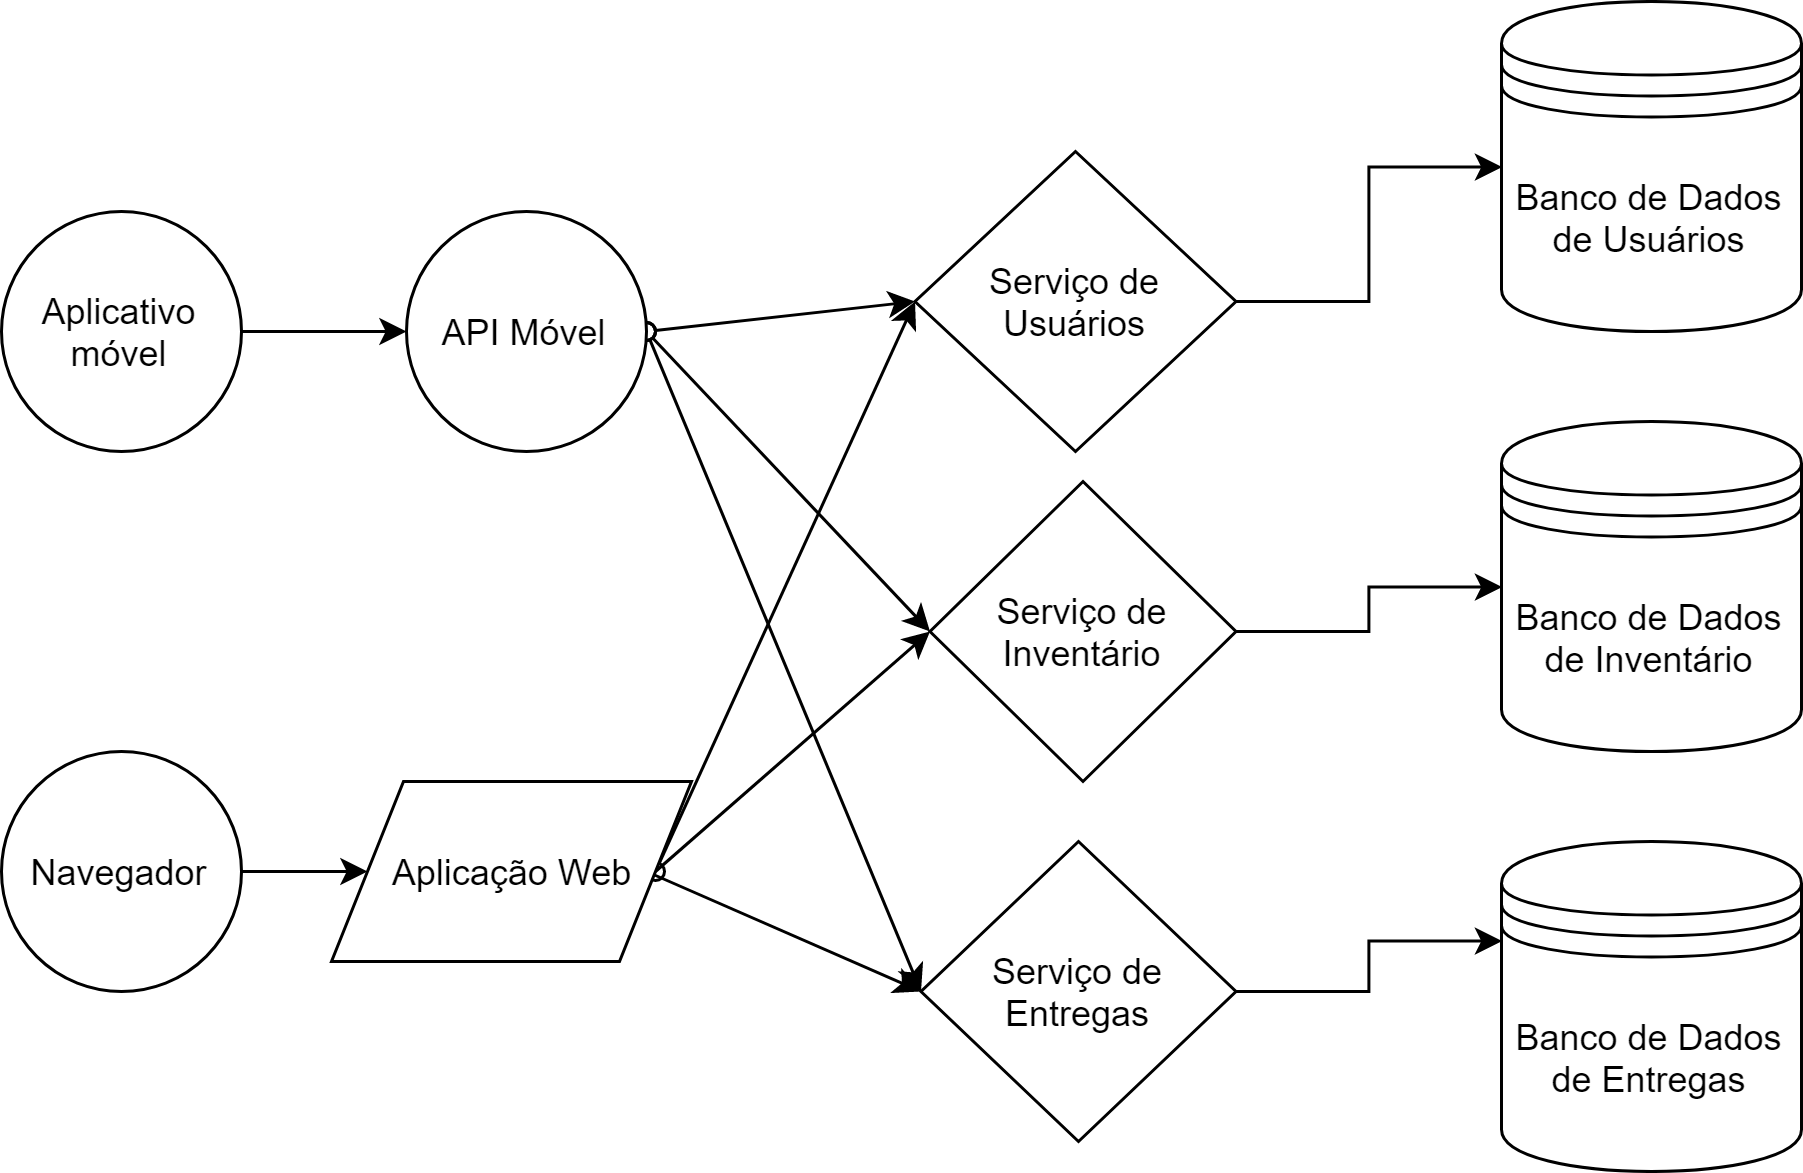
\includegraphics[width=1\linewidth]{figuras/microservices.png}
	\caption{Exemplo arquitetura de microsserviços.}
	\label{fig:arquitetura-microsservicos}
\end{figure}

Microsserviços são os resultados da decomposição funcional de uma aplicação. São caracterizados pela definição de sua interface e função no sistema. Como cada serviço deve ser independente, uma alteração na sua implementação não deve afetar o funcionamento dos demais. \cite{Pahl}

\subsection{Protocolo de comunicação MQTT}

MQTT significa \textit{Message Queuing Telemetry Transport}, traduzido para o português como Transporte de Telemetria de Enfileiramento de Mensagens. É um protocolo de transporte leve que otimiza o uso da a largura de banda de rede\footnote{\url{http://public.dhe. ibm.com/software/dw/webservices/ws-mqtt/mqtt-v3r1.html}}. O MQTT trabalha sobre o protocolo TCP e garante a entrega de mensagens de um nó para um servidor. Sendo um protocolo orientado por troca de mensagens, MQTT é ideal para aplicações IoT, que comumente tem recursos e capacidades limitados.

É um protocolo inicialmente desenvolvido pela IBM\footnote{\url{http://www.hivemq.com/blog/mqtt-essentials-part-1-introducing-mqtt}} em 1999, sendo recentemente reconhecido como padrão pela OASIS (Organizarion for the Advancement of Structured Information Standards)\footnote{\url{https://www.oasis-open.org/news/announcements/ mqtt-version-3-1-1-becomes-an-oasis-standard}}.

\citeauthor{Kodali2017} (\citeyear{Kodali2017}) definiu o MQTT como um protocolo baseado em \textit {publisher/subscriber}. Qualquer conexão MQTT envolve dois tipos de agentes, os clientes e um \textit {broker}, ou servidor. Qualquer dispositivo ou programa que é conectado pela rede e troca mensagens através do MQTT é chamado de cliente. Um cliente pode ser tanto um \textit {publisher} e/ou um \textit {subscriber}. Um \textit {publisher} publica mensagens e um \textit {subscriber} requisita o recebimento de mensagens. Um MQTT \textit {server} é um programa que interconecta os clientes. Ele aceita e transmite as mensagens através de múltiplos clientes conectados à ele.

\begin{figure}[htbp]
	\centering
	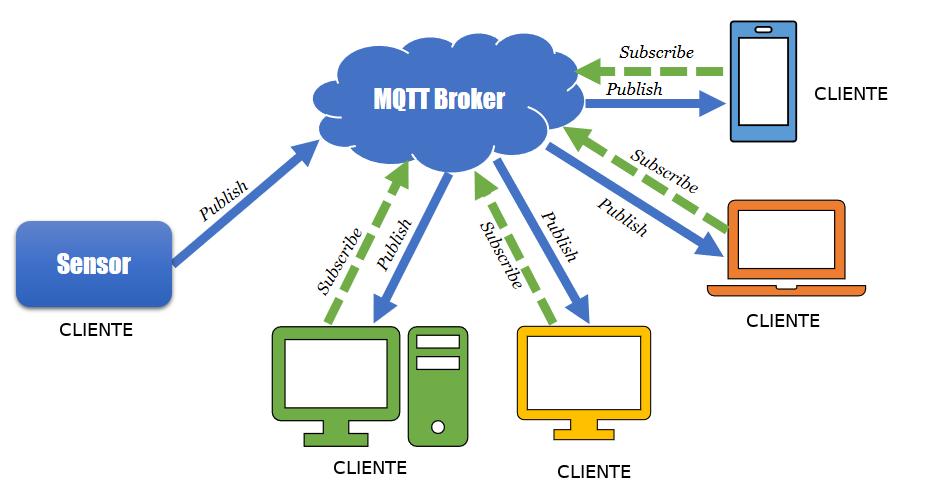
\includegraphics[width=1\linewidth]{figuras/mqtt-architecture.png}
	\caption{Exemplo da arquitetura do MQTT.}
	\legend{Fonte: \citeauthor{embeddedmqtt} (\citeyear{embeddedmqtt})}
	\label{fig:arquitetura-mqtt}
\end{figure}

\newpage

Dispositivos como sensores e celulares podem ser vistos como clientes do ponto de vista da arquitetura MQTT. Quando um cliente tem alguma informação para transmitir, ele publica o dado para o \textit {broker}.

A Figura \ref{fig:arquitetura-mqtt} apresenta um exemplo de arquitetura MQTT comum. O \textit {broker} MQTT, ou servidor MQTT é responsável por coletar e organizar os dados. As mensagens publicadas por clientes MQTT são transmitidas para outros clientes MQTT que se inscreverem ao tópico. O MQTT é desenhado para simplificar a implementação no cliente por concentrar todas as complexidades no \textit {broker}. Os \textit {publishers} e \textit {subscribers} são isolados, o que significa que eles não precisam conhecer a existência do outro.

\subsubsection{MQTT Mosquitto}

O Mosquitto é um \textit{broker} MQTT de código aberto \cite{Kodali2017} que entrega uma implementação de servidor e cliente MQTT. Utiliza o modelo \textit{publisher/subscriber}, tem uma baixa utilização de rede e pode ser implementado em dispositivos de baixo custo como microcontroladores. \cite{Light}

Segundo \citeauthor{Light} (\citeyear{Light}), Mosquitto é recomendado para o uso sempre em que se necessita de mensagens leves, particularmente em dispositivos com recursos limitados.

O Projeto Mosquitto é um membro da Eclipse Foundation. Existem três partes no projeto:

\begin{itemize}
	\item O servidor principal Mosquitto.
	\item Os clientes mosquitto \textit{pub} e mosquitto \textit{sub}, que contém ferramentas para se comunicar com o servidor MQTT.
	\item Uma biblioteca cliente MQTT, escrita em C.
\end{itemize}

%\subsection{Docker}
%
%Docker é um projeto \textit{open source} que foi inicialmente lançado em 2013, atraiu grande atenção na industria de TI. É uma plataforma de conteinerização que possibilita usuários a construir sua aplicação dentro de um conteiner e transferir conteiners através de máquinas com diferentes sistemas operacionais de um jeito simples. \cite{chang2017kubernetes}
%
%Existem três componentes principais do Docker:
%
%\begin{itemize}
%	\item \textit{Docker images}: são \textit{templates} de leitura que servem como base para a criação de conteiners.;
%	\item \textit{Docker registries}: é o local onde estão uma grande coleção de \textit{Docker images}.;
%	\item \textit{Docker containers}: são as instâncias virtuais em que as aplicações estão rodando. Cada conteiner contem uma aplicação rodando e todas os seus arquivos de dependências, como o código, bibliotecas e utilitários do sistema.
%\end{itemize}
%
%A construção de imagens pode ser feita de duas maneiras. É possível criar um conteiner através de uma imagem já existente (\textit{docker run}), realizar modificações e instalações dentro do conteiner, parar o container e depois salvar o estado atual do conteiner como uma nova imagem (\textit{docker commit}). Este processo é parecido com uma instalação clássica de uma máquina virtual, mas deve ser feito para cada imagem caso haja alguma atualização, já que as imagens são padronizadas. Para automatizar o processo, \textit{Dockerfiles} nos permite especificar uma imagem de base e uma sequência de comandos que serão executados quando a imagem é construída, juntamente com outras opções de especificações, como portas a serem expostas. A imagem é depois construída com o comando \textit{docker build}.\cite{DiPietro}
